\section{Results}

Fig. \ref{fig:results} shows the achieved performance for different problem sizes on all three kernels.
NanoVDB achieves overall better results on the CPU compared to OpenVDB. 
Above one million rays the GPU starts to overtake both CPU kernels.

OpenVDB achieves up to 18.5 MRps \footnote{1 MRps = $10^6$ Rays per second}. NanoVDB consistently outperforms OpenVDB and reaches up to 29.7 MRps.
For problems with 1 million rays or more the GPU kernel overtakes both CPU implementations and achieves up to 117.4 MRps.
Therefore the switch from OpenVDB to NanoVDB increased performance by a factor of 6.3.
 
Furthermore both CPU implementations suffer from random drops in performance while GPU results are more consistent. 


\begin{figure}[h]
    % Rigth image
    \begin{subfigure}{0.5\textwidth}
    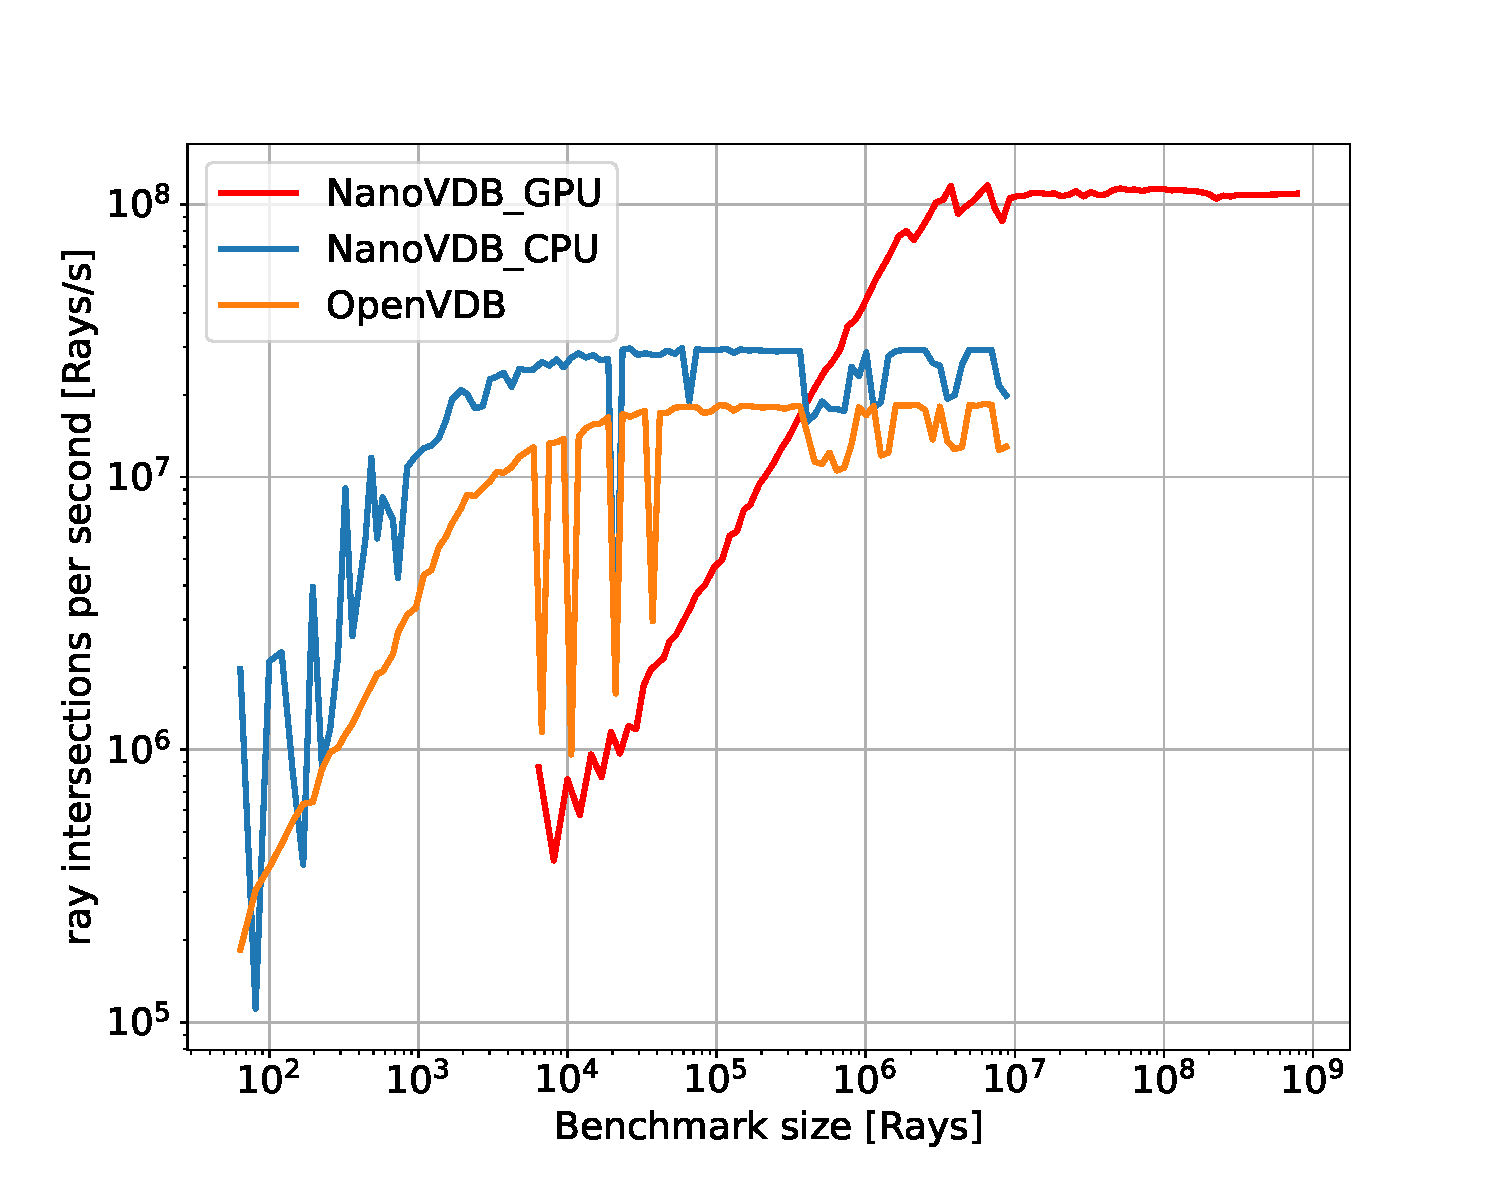
\includegraphics[width=1\linewidth]{res/results.pdf} 
    \caption{}
    %\label{fig:serial-solution}
    
\end{subfigure}
    % left image
    \begin{subfigure}{0.4\textwidth}
    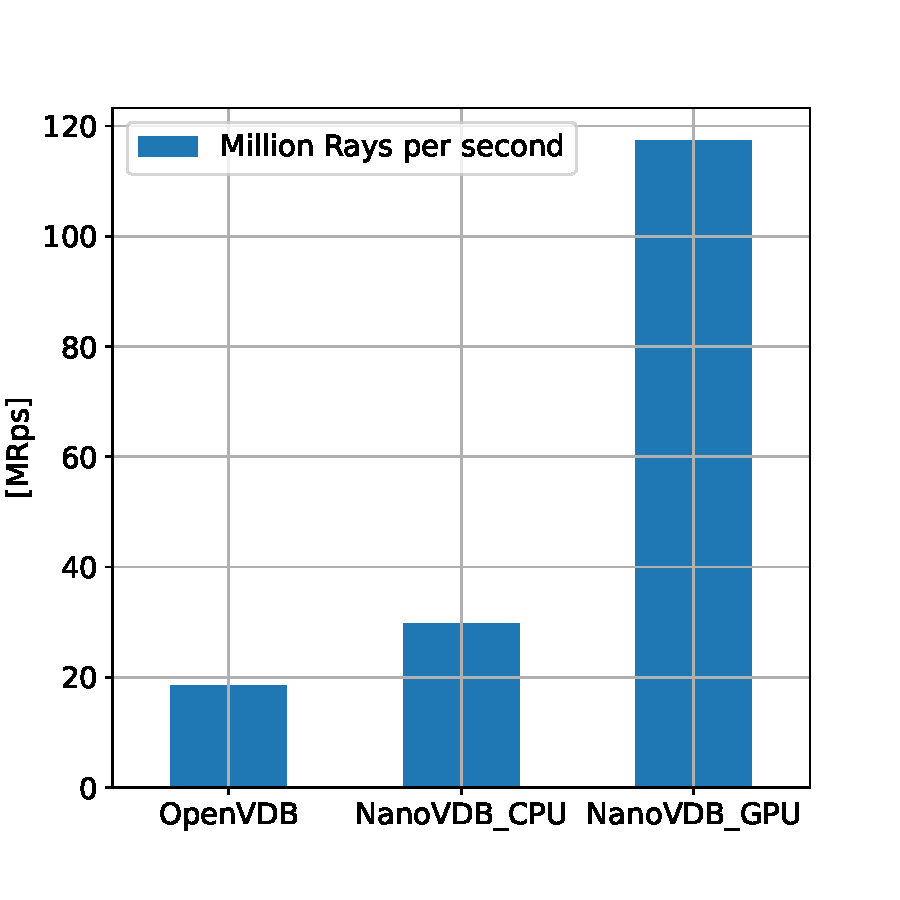
\includegraphics[width=1\linewidth]{res/barplot.pdf}
    \caption{}
    %\label{fig:parallel-solution}
\end{subfigure}

\caption{\textbf{a} measured performance across different problem sizes. \textbf{b} Best results for each kernel}
\label{fig:results}
\end{figure}


\nocite{openvdb}
\nocite{nanovdb}
